\documentclass[11pt]{article}

\usepackage[margin=0.85in]{geometry}
\usepackage{float}
\setlength{\textfloatsep}{6pt plus 2pt minus 2pt}
\setlength{\intextsep}{4pt plus 2pt minus 2pt}
\setlength{\floatsep}{6pt plus 2pt minus 2pt}
\setlength{\abovecaptionskip}{3pt}
\setlength{\belowcaptionskip}{1pt}
\setlength{\parskip}{1pt}
\renewcommand{\baselinestretch}{0.97}
\renewcommand{\arraystretch}{0.95}
\makeatletter
\renewcommand\section{\@startsection{section}{1}{\z@}%
  {-1.5ex \@plus -0.5ex \@minus -.2ex}%
  {0.8ex \@plus.2ex}%
  {\normalfont\large\bfseries}}
\renewcommand\subsection{\@startsection{subsection}{2}{\z@}%
  {-1.2ex\@plus -0.5ex \@minus -.2ex}%
  {0.5ex \@plus .2ex}%
  {\normalfont\normalsize\bfseries}}
\makeatother
\usepackage{amsmath}
\usepackage{amssymb}
\usepackage{graphicx}
\usepackage{booktabs}
\usepackage{array}
\usepackage{microtype}
\usepackage{caption}
\usepackage{natbib}
\usepackage{hyperref}
\usepackage{url}

\bibliographystyle{plainnat}

\graphicspath{{../figures/}}

\hypersetup{
  colorlinks=true,
  linkcolor=black,
  citecolor=black,
  urlcolor=blue
}

\newcommand{\mF}{macro-F1}

\title{An Audited Comparison of TabNet and XGBoost on NOAA Storm Events:\\
       A Pre-Registered Negative Result with Temporal-Split Qualification}
\author{Nathaniel Black \and Dhruv Patel \and Marcos Diaz Vazquez}
\date{}

\begin{document}
\maketitle

%======================================================================
\begin{abstract}
We pre-registered the hypothesis that TabNet's sequential attention
would outperform a tuned gradient-boosted baseline on a high-volume,
low-feature severe-weather classification task (NOAA Storm Events
2023; 117{,}717 records after filtering to ten event classes; 8
engineered features from 51 raw columns). On the principal
random-split, iid evaluation the hypothesis is falsified along every
axis we tested: tuned XGBoost reaches \mF{} 0.9001 against refined
TabNet's 0.8513, a paired-bootstrap gap of $+0.049$ (95\% CI
$[+0.044, +0.054]$; McNemar $\chi^2 = 591.6$, $p < 10^{-130}$),
with the largest per-class losses on Hail and Thunderstorm Wind ---
the boundary classes the proposal had singled out. A surface read
of Expected Calibration Error initially favored TabNet (0.0043 vs
0.0250), but a three-control audit overturns that reading: Brier and
NLL both favor XGBoost decisively, and a single learned temperature
$T = 1.26$ brings XGBoost below TabNet on ECE as well, without
changing the \mF{} result. On a 2023$\rightarrow$2024 temporal fold,
TabNet's softer fit degrades 3--4$\times$ less than XGBoost's on
Hail and Thunderstorm Wind --- the one place the proposal's prediction
is partially recovered. We report this as a robust negative result
against an attention-based tabular DL method in a low-feature regime,
with a methodological caution against ECE-only calibration claims.
\end{abstract}

%======================================================================
\section{Introduction}\label{sec:intro}

A persistent question in applied tabular machine learning is whether
attention-based deep architectures can outperform gradient-boosted
tree ensembles on the kind of structured, finite-feature,
high-volume classification problems that account for most real-world
tabular workloads. The two methodological poles are well-defined:
XGBoost \citep{chen2016xgboost} is the de-facto baseline, with
split-finding heuristics that have been refined over a decade of
competition and production use; TabNet \citep{arik2021tabnet} is the
most prominent attention-based alternative, with a sequential
decision process that learns sparse per-instance feature masks at
each of several steps. The broader literature reviewing this
comparison has reached mixed verdicts: \citet{grinsztajn2022why}
report that tree-based methods remain strictly better on most
tabular benchmarks, while \citet{shwartz2022tabular} caution that no
single tabular DL method consistently beats well-tuned trees across
heterogeneous tasks. Our work sits inside that debate and
contributes a single high-volume, low-feature, multi-class
operational case study with statistical testing, a calibration
audit, and a temporal-shift qualification.

The dataset is the NOAA Storm Events database (2023--2024), filtered
to the ten most frequent event-type classes --- Drought, Excessive
Heat, Flash Flood, Flood, Hail, Heat, High Wind, Marine Thunderstorm
Wind, Thunderstorm Wind, and Winter Weather --- for 117{,}717
training-evaluation records and a 55{,}061-record 2024 hold-out. The
raw archive exposes 51 columns; after feature engineering
(\S\ref{sec:data}) the working set is 8 features mixing categorical
event-context codes (\texttt{CZ\_TYPE\_ENC}, \texttt{STATE\_ENC},
\texttt{WFO\_ENC}), continuous time-of-event variables
(\texttt{HOUR}, \texttt{MONTH}, \texttt{DURATION\_MIN}), and
geographic coordinates (\texttt{BEGIN\_LAT}, \texttt{BEGIN\_LON}).
We pre-registered the hypothesis that TabNet's sparse attention
would outperform a tuned XGBoost baseline on this task, with the
largest gains expected on the two boundary classes Hail vs
Thunderstorm Wind whose feature distributions overlap most.

The paper makes three contributions.
\textbf{(1)~A statistically tested comparison} of a tuned XGBoost
baseline against a two-stage tuned TabNet on both a random-split
iid test fold and a 2023$\rightarrow$2024 temporal hold-out. The
random-split result falsifies the pre-registered hypothesis
decisively: XGBoost 0.9001 vs TabNet 0.8513 (bootstrap diff $+0.049$,
95\% CI $[+0.044, +0.054]$; McNemar $\chi^2 = 591.6$,
$p < 10^{-130}$), with XGBoost ahead on every per-class F1.
\textbf{(2)~A calibration audit} that treats an apparent
TabNet ECE advantage as a hypothesis to audit and runs three
controls (proper scoring rules, temperature scaling, argmax
invariance); the audit overturns the ECE finding and yields the
methodological caution that ECE-only calibration claims should be
paired with at least one proper scoring rule and a
temperature-scaling baseline.
\textbf{(3)~A temporal-split qualification} on the proposal's named
boundary classes: under 2023$\rightarrow$2024 shift TabNet beats
XGBoost on Hail ($+0.037$ F1) and Thunderstorm Wind ($+0.017$),
with per-class F1 drops 3--4$\times$ smaller. We report this as a
substantive qualification, not a thesis reversal --- one annual
fold is too thin a base for a domain-shift claim
(\S\ref{sec:limitations}).

%======================================================================
\section{Related Work}\label{sec:relwork}

Our work touches four threads. \textbf{Attention-based tabular DL.}
TabNet \citep{arik2021tabnet} is the canonical
sequential-attention architecture for structured data: at each of
$N$ decision steps an attentive transformer learns a sparse,
instance-adaptive mask over features, regularized by a sparsity
prior $\gamma$. Follow-on methods (FT-Transformer, SAINT, NODE)
inherit the same selection-driven motivation.
\textbf{Gradient-boosted baselines.} XGBoost \citep{chen2016xgboost}
remains the long-standing reference for tabular classification; its
weighted-quantile sketch and histogram-based extensions
(LightGBM, CatBoost) set the accuracy bar against which tabular DL
methods are reported. \textbf{The tabular-DL-vs-trees debate.}
\citet{grinsztajn2022why} benchmark a wide range of tabular DL
methods and report tree-based methods remain strictly better on
most; \citet{shwartz2022tabular} reach a complementary conclusion,
flagging the gap as most pronounced when the input feature set is
small and free of irrelevant features --- exactly our regime, on
which \S\ref{sec:discussion} hangs its mechanism claim.
\textbf{Calibration.} \citet{guo2017calibration} is the standard
reference on neural-classifier miscalibration: modern deep
classifiers are systematically overconfident, ECE is a useful but
imperfect scalar, and a single learned temperature is a strong
post-hoc correction. Our \S\ref{sec:audit} audit treats ECE, Brier,
NLL, and temperature scaling jointly in that spirit, generalizing
the caution to the \emph{under}-confident case as well.

We are not aware of prior work that pairs a pre-registered
TabNet-vs-XGBoost comparison on NOAA Storm Events with a
statistical-test-anchored \mF{} result, a three-control calibration
audit, and a temporal-shift qualification on named boundary classes.

%======================================================================
\section{Data}\label{sec:data}

\subsection{Source}

We used the NOAA Storm Events Database for calendar years 2023 and
2024, downloaded from the National Centers for Environmental
Information FTP archive
(\texttt{StormEvents\_details-ftp\_v1.0\_d2023} and the 2024 release
of the same table). Each row in the raw archive represents one
reported severe-weather event and carries 51 columns covering
identifiers, temporal fields, geographic fields, magnitude and
damage estimates, and the categorical \texttt{EVENT\_TYPE} label
that we treat as the classification target. The 51 raw-column count
is what we use to satisfy the project's high-volume tabular data
requirement at the source level; the working feature set described
below is a smaller, engineered subset.

\subsection{Filtering and retained classes}

The raw \texttt{EVENT\_TYPE} vocabulary in the NOAA archive contains
dozens of categories with a heavy long tail. We restricted the
analysis to the ten most frequent event types in the combined
2023~+~2024 archive, which together account for 117{,}717 records.
The retained classes are shown in Figure~\ref{fig:class-dist} and
listed in Table~\ref{tab:classes}.

\begin{table}[h]
  \centering
  \small
  \caption{Retained event classes and their counts in the combined
  2023~+~2024 dataset.}
  \label{tab:classes}
  \begin{tabular}{lrr}
    \toprule
    class & combined $N$ & share \\
    \midrule
    Thunderstorm Wind         & 41{,}177 & 35.0\% \\
    Hail                      & 20{,}702 & 17.6\% \\
    Drought                   &  9{,}288 &  7.9\% \\
    Flash Flood               &  8{,}286 &  7.0\% \\
    Excessive Heat            &  7{,}684 &  6.5\% \\
    High Wind                 &  7{,}485 &  6.4\% \\
    Heat                      &  6{,}494 &  5.5\% \\
    Winter Weather            &  6{,}448 &  5.5\% \\
    Flood                     &  5{,}318 &  4.5\% \\
    Marine Thunderstorm Wind  &  4{,}835 &  4.1\% \\
    \midrule
    \textbf{total}            & \textbf{117{,}717} & 100\% \\
    \bottomrule
  \end{tabular}
\end{table}

The distribution is moderately imbalanced --- Thunderstorm Wind
alone covers a third of the dataset and the bottom six classes each
fall below 8\%. We report \mF{} throughout as the headline metric so
the long-tail classes are not drowned out by Thunderstorm Wind, and
we do not apply class-reweighting to either model so the comparison
is a like-for-like test of representation rather than of
loss-weighting tricks.

\subsection{Feature engineering}

We engineered eight features from the raw schema: \texttt{MONTH}
(1--12 from \texttt{MONTH\_NAME}), \texttt{HOUR} (extracted from the
four-digit \texttt{BEGIN\_TIME}), \texttt{DURATION\_MIN} (the
difference between \texttt{END\_DATE\_TIME} and
\texttt{BEGIN\_DATE\_TIME} in minutes), \texttt{BEGIN\_LAT} and
\texttt{BEGIN\_LON} (event-onset coordinates), \texttt{CZ\_TYPE\_ENC}
(a binary indicator for County vs Zone reporting), and label-encoded
\texttt{STATE\_ENC} and \texttt{WFO\_ENC} (state code and NWS
Forecast Office). All eight features are shared by both models so
the XGBoost-vs-TabNet comparison is not confounded by feature
availability.

The working set is deliberately small: the raw NOAA columns are
dominated by sparse free-text and post-event damage estimates that
leak label-correlated information at training time, and the 8-feature
regime makes the central question interesting because TabNet's
design advantage is attention-based feature \emph{filtering}
(\S\ref{sec:discussion}).

\subsection{Splits}

We evaluated each model under two splits.

\paragraph{Random split.} A single 80/20 stratified split over the
combined 2023~+~2024 dataset, with \texttt{random\_state = 42}. The
train fold has 94{,}173 rows and the test fold has 23{,}544 rows.
All headline numbers in \S\ref{sec:experiments}, \S\ref{sec:stats},
and \S\ref{sec:audit} are computed on this test fold unless
otherwise stated.

\paragraph{Temporal split.} A pre-registered out-of-time evaluation
in which the 2023 archive is the train fold (62{,}656 rows) and the
2024 archive is the test fold (55{,}061 rows). The class supports
differ markedly between random and temporal test folds because 2024
saw a substantially higher Thunderstorm Wind and Hail count than the
dataset average; this is an artifact of inter-annual variability in
severe-weather frequency, not of our split construction. The
temporal split exists to test generalization under year-to-year
distribution shift, and we report it alongside the random-split
numbers in \S\ref{sec:experiments} and \S\ref{sec:errors}.

\subsection{Missing-value treatment}

\texttt{BEGIN\_LAT}/\texttt{BEGIN\_LON} are missing for a substantial
fraction of records. We impute on the \emph{training} rows only with
a three-level hierarchical median fill
(\texttt{(STATE, CZ\_FIPS)} $\rightarrow$ \texttt{(STATE, WFO)}
$\rightarrow$ \texttt{STATE}). An ablation on a drop-NaN variant
moved XGBoost \mF{} by $< 6 \times 10^{-5}$ and TabNet \mF{} by
$+0.022$ in favor of imputation; we report impute throughout. No
other feature contains missing values.

\begin{figure}[!htbp]
  \centering
  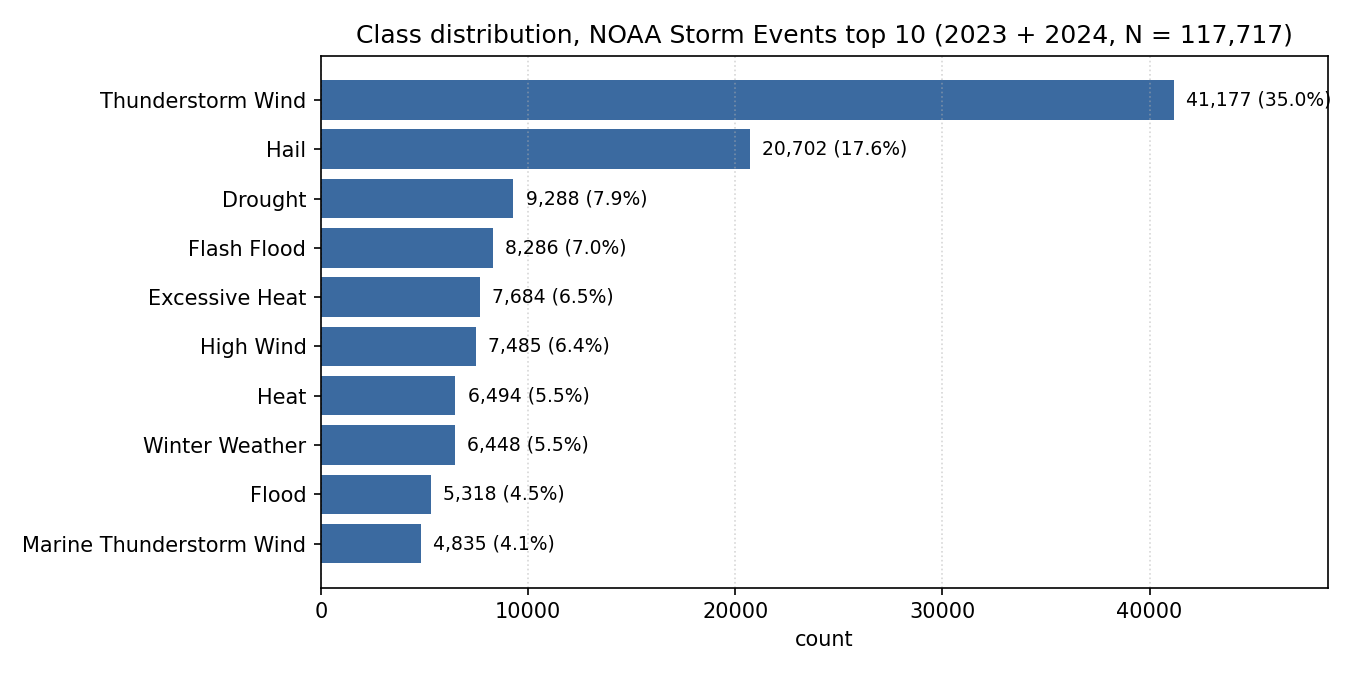
\includegraphics[width=0.55\textwidth]{class_distribution.png}
  \caption{Class distribution on the combined 2023~+~2024 retained-
  class dataset ($N = 117{,}717$). Thunderstorm Wind is the modal
  class at $\sim$35\%; Hail second at $\sim$18\%; the remaining
  eight classes share the long tail.}
  \label{fig:class-dist}
\end{figure}

%======================================================================
\section{Methods}\label{sec:methods}

\subsection{Models and hyperparameter selection}\label{sec:methods-models}

\paragraph{XGBoost baseline.} XGBoost~3.2 with the \texttt{hist}
tree method and \texttt{multi:softmax} objective. Hyperparameters
were chosen by a 192-candidate 5-fold stratified grid search
(\texttt{StratifiedKFold(n\_splits=5, shuffle=True,
random\_state=42)}, \texttt{scoring='f1\_macro'}) over
\texttt{learning\_rate} $\in \{0.01, 0.05, 0.1, 0.3\}$,
\texttt{max\_depth} $\in \{3, 5, 7, 9\}$,
\texttt{n\_estimators} $\in \{100, 300, 500, 700\}$, and
\texttt{subsample} $\in \{0.7, 0.8, 1.0\}$. The selected
configuration was \texttt{(0.1, 9, 500, 0.7)} with CV \mF{} 0.8949;
refit on the full training fold for evaluation.

\paragraph{TabNet.} \texttt{pytorch\_tabnet 4.x}
\citep{arik2021tabnet}. The baseline configuration uses
out-of-the-box defaults ($n_d = n_a = 8$, $n_{\mathrm{steps}} = 3$,
$\gamma = 1.3$, $lr = 0.02$, $\mathrm{batch\_size} = 1024$, Adam with
StepLR, 100 epochs, \texttt{patience = 15}) and posts random-split
\mF{} 0.7828. Tuning then proceeded in two stages:
(i)~a 27-config coarse sweep over $n_d = n_a, n_{\mathrm{steps}},
lr$ on a held-out validation split, selecting $(16, 7, 0.02)$
(val \mF{} 0.8358); (ii)~a 12-config refined sweep over
$\gamma \in \{1.0, 1.3, 1.5, 1.8\}$ and
$\mathrm{batch\_size} \in \{512, 1024, 2048\}$ with 3-fold CV,
selecting $\gamma = 1.0$ and $\mathrm{batch\_size} = 1024$
(CV \mF{} $0.8298 \pm 0.0076$). Refit on the full training fold,
the refined TabNet scores \mF{} 0.8513.

\paragraph{Protocol caveat.}\label{sec:methods-protocol} The random-split
results use the refined TabNet. The temporal-split results use the
coarse-sweep configuration ($\gamma = 1.3$): the refined finding was
locked after the temporal fit had already been run, and we chose not
to re-run on CUDA. Any temporal per-class advantage TabNet shows is
therefore a lower bound on what a re-tuned TabNet would deliver
(\S\ref{sec:discussion}).%
\footnote{All random-seeded operations use
\texttt{random\_state = 42}. TabNet does not seed PyTorch globally,
so its runs are reproducible up to GPU non-determinism; the
random-split \mF{} reproduced within rounding across coarse, tuned,
and refined refits. All test predictions and probabilities are
persisted so every downstream analysis runs from frozen artifacts on
CPU.}

\subsection{Evaluation metrics}

We report \mF{} as the primary metric and macro one-versus-rest
ROC-AUC as a secondary discrimination metric. For probabilities we
report Expected Calibration Error (10 equal-width bins on the
maximum-class confidence per \citealp{guo2017calibration}),
Brier score, and negative log-likelihood. Statistical comparisons
in \S\ref{sec:stats} use a paired bootstrap on the \mF{} difference
(1{,}000 resamples, paired by test-row index) and a
continuity-corrected McNemar test on per-row correctness.

%======================================================================
\section{Experiments}\label{sec:experiments}

This section reports the locked headline numbers under both splits
and both models. Per-row statistical testing is deferred to
\S\ref{sec:stats}; per-class and error-overlap analyses to
\S\ref{sec:errors}; calibration and probability quality to
\S\ref{sec:audit}.

\subsection{Random-split macro-F1}\label{sec:exp-mf1}

We report four configurations on the random-split test fold
(23{,}544 rows): a default-hyperparameter XGBoost, the tuned XGBoost
selected in \S\ref{sec:methods-models}, the baseline TabNet, and
the refined TabNet selected in \S\ref{sec:methods-models}.

\begin{center}
\small
\begin{tabular}{lr}
\toprule
model & test \mF{} \\
\midrule
default XGBoost                  & 0.8887 \\
\textbf{tuned XGBoost}           & \textbf{0.9001} \\
baseline TabNet                  & 0.7828 \\
TabNet (coarse-sweep best)       & 0.8231 \\
\textbf{refined TabNet}          & \textbf{0.8513} \\
\bottomrule
\end{tabular}
\end{center}

The two bolded rows are the configurations we treat as the final
models. Tuning helped TabNet more in absolute terms ($+0.0685$
\mF{}) than XGBoost ($+0.0114$); the baseline XGBoost is already
close to its tuned ceiling. The tuned XGBoost outperforms the
refined TabNet by 0.0488 \mF{}: on the random split, by the
\mF{} metric, the pre-registered hypothesis is falsified ---
\S\ref{sec:stats} confirms the falsification is statistically
robust.

\subsection{Discrimination by ROC-AUC}\label{sec:exp-auc}

Macro one-versus-rest ROC-AUC tracks the \mF{} ordering with a
narrower spread: tuned XGBoost 0.9907, refined TabNet 0.9831
(baseline TabNet 0.9760, default XGBoost 0.9882). The AUC gap
(0.0076) is smaller than the \mF{} gap (0.0488) because AUC scores
the model on its \emph{ranking} of probabilities rather than its
hard-labeling: TabNet's softer predictions (\S\ref{sec:audit}) rank
classes correctly more often than they confidently top-1 the right
class. The \mF{} result is the one the proposal commits to and the
one we treat as the headline. The lowest one-vs-rest AUC under
either model is Hail (TabNet's 0.927), one of the two proposal
boundary classes \S\ref{sec:errors} returns to.

\subsection{Temporal generalization, 2023\,$\rightarrow$\,2024}\label{sec:exp-temporal}

We re-trained both models on the 2023 archive only (62{,}656 rows)
and evaluated on the 2024 archive (55{,}061 rows), holding all
hyperparameters fixed at the values selected in
\S\ref{sec:methods} (with the \S\ref{sec:methods-protocol} caveat
that TabNet on the temporal split uses the coarse-sweep
configuration, not the refined one).

\begin{center}
\small
\begin{tabular}{lrrr}
\toprule
model & random \mF{} & temporal \mF{} & $\Delta$ (temporal $-$ random) \\
\midrule
tuned XGBoost                       & 0.9001 & 0.7556 & $-0.1445$ \\
TabNet (coarse temporal config)     & 0.8231 & 0.7487 & $-0.0744$ \\
\bottomrule
\end{tabular}
\end{center}

The temporal split is harder for both models. The aggregate gap
between the two narrows substantially: from 0.0488 \mF{} on the
random split (refined TabNet vs tuned XGBoost; using the
matched coarse-config TabNet the gap on the random split is 0.0770)
to 0.0069 on the 2023$\rightarrow$2024 split. On the aggregate
metric XGBoost still wins, but only just; the narrowing is driven by
XGBoost dropping further under shift than TabNet does. We do not
promote this aggregate narrowing to a thesis --- the per-class
breakdown in \S\ref{sec:errors} shows the narrowing concentrates in
two specific classes, and one annual fold is not enough to make a
domain-adaptation claim. But the contrast between the two
$\Delta$-columns ($-0.1445$ vs $-0.0744$) is itself worth flagging:
TabNet's softer fit appears to generalize more gracefully across
years on this dataset, and \S\ref{sec:discussion} takes that as a
hypothesis-of-mechanism consistent with the \S\ref{sec:audit}
calibration audit.

\begin{figure}[!htbp]
  \centering
  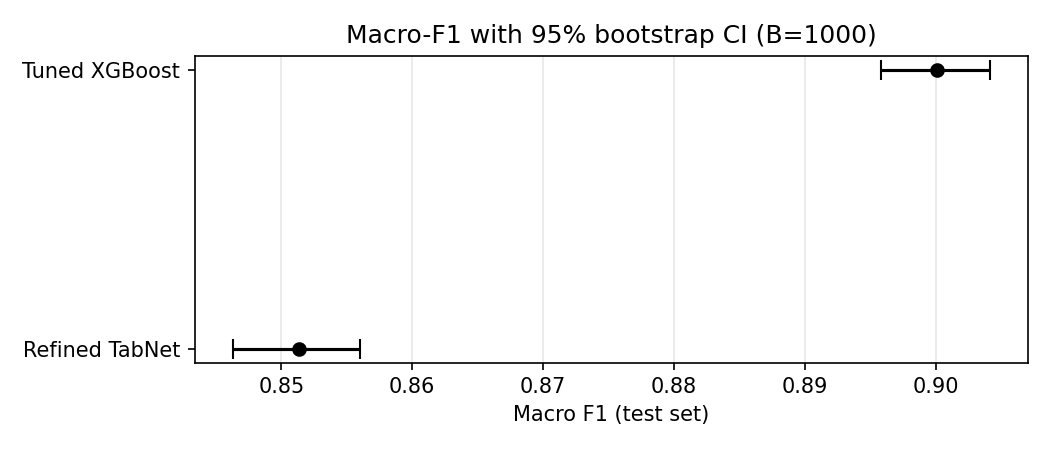
\includegraphics[width=0.5\textwidth]{macro_f1_with_ci.png}
  \caption{\mF{} on the random-split test fold for the tuned XGBoost
  and the refined TabNet, with 95\% paired-bootstrap confidence
  intervals. The intervals are disjoint at every resample; the
  bootstrap difference is $+0.0489$ in XGBoost's favor with 95\% CI
  $[+0.0444, +0.0536]$.}
  \label{fig:mf1-ci}
\end{figure}

\begin{figure}[!htbp]
  \centering
  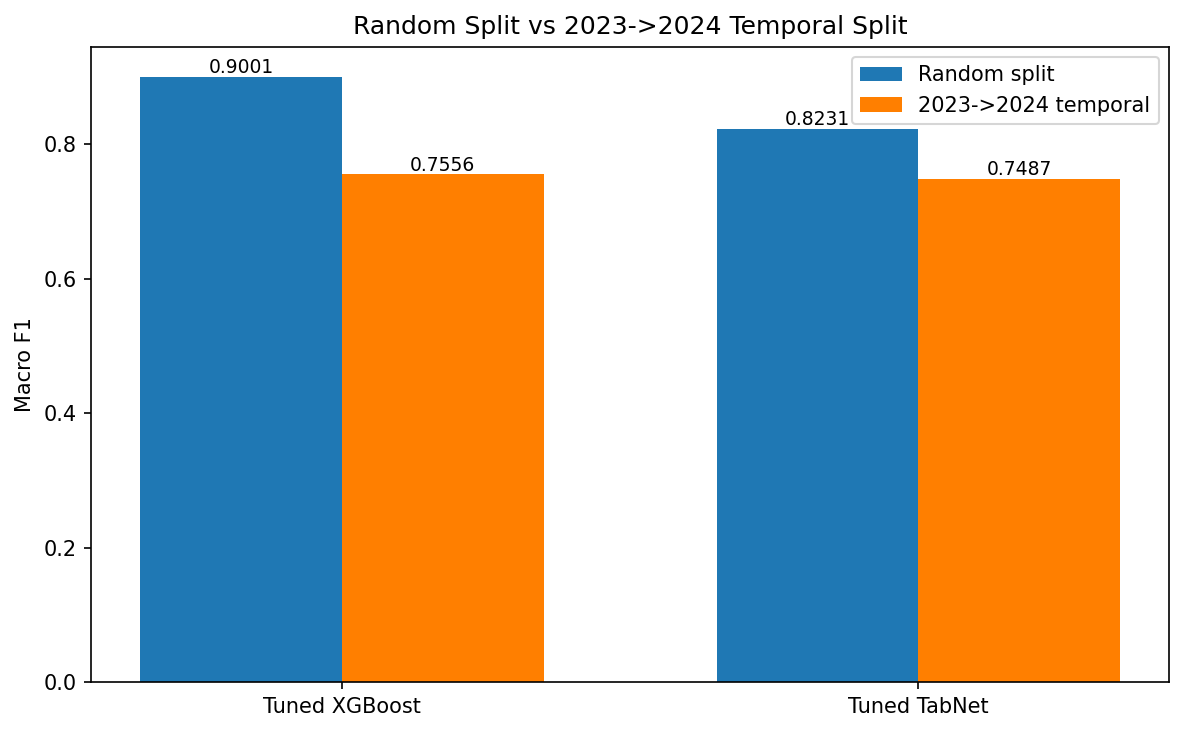
\includegraphics[width=0.5\textwidth]{random_vs_temporal_split.png}
  \caption{\mF{} under the random split and the
  2023$\rightarrow$2024 temporal hold-out. The temporal gap (0.0069)
  is much narrower than the random-split gap (0.0488) because
  XGBoost drops further under shift.}
  \label{fig:rand-vs-temp}
\end{figure}

%======================================================================
\section{Statistical Analysis}\label{sec:stats}

The point-estimate gap of 0.0488 \mF{} between tuned XGBoost and the
refined TabNet on the random-split test fold
(\S\ref{sec:exp-mf1}) admits two reads: it could reflect a real
difference in model behavior, or it could be within the noise we
should expect from a 23{,}544-row test fold. We address the question
with two complementary tests: a paired bootstrap on the \mF{}
difference and a McNemar test on per-row correctness.

\subsection{Paired bootstrap on macro-F1}

We drew 1{,}000 paired bootstrap resamples from the random-split
test fold (\texttt{seed = 42}). Each resample drew test-row indices
with replacement and computed \mF{} for both models using the
\emph{same} sampled indices, so the resampled distributions are
jointly correlated.

\begin{center}
\small
\begin{tabular}{lr}
\toprule
quantity & value \\
\midrule
XGBoost \mF{} (point)        & 0.9001 \\
XGBoost \mF{} 95\% CI        & $[0.8958, 0.9041]$ \\
TabNet \mF{} (point)         & 0.8513 \\
TabNet \mF{} 95\% CI         & $[0.8463, 0.8560]$ \\
paired diff (XGB $-$ TabNet), mean & $+0.0489$ \\
paired diff 95\% CI          & $[+0.0444, +0.0536]$ \\
two-sided $p$-value          & $< 10^{-3}$ \\
\bottomrule
\end{tabular}
\end{center}

The two model-level confidence intervals are disjoint. The 95\% CI
on the paired difference is well to the right of zero, and not a
single one of the 1{,}000 resamples produced a TabNet-favoring
difference, so the two-sided empirical $p$-value is 0 to the
resolution of our resample count (reported as $< 10^{-3}$). The
bootstrap mean diff ($+0.0489$) sits within 0.0001 of the
point-estimate diff ($+0.0488$), so resampling is not introducing
any noticeable bias.

\subsection{McNemar on per-row correctness}

We tabulate the joint correctness of the two models against the
ground-truth labels on the 23{,}544-row test fold.

\begin{center}
\small
\begin{tabular}{lrrr}
\toprule
                       & XGB correct & XGB wrong & row total \\
\midrule
\textbf{TabNet correct} & 18{,}419 &    908 & 19{,}327 \\
\textbf{TabNet wrong}   &  2{,}283 &  1{,}934 &  4{,}217 \\
\textbf{column total}   & 20{,}702 &  2{,}842 & 23{,}544 \\
\bottomrule
\end{tabular}
\end{center}

With continuity correction the McNemar statistic is $\chi^2 = 591.6$
on 1 d.f., $p \approx 1.1 \times 10^{-130}$. The asymmetry between
the off-diagonals is large and in XGBoost's favor: there are roughly
2.5 rows that only XGBoost gets right for every row that only
TabNet does.

Both tests reject the null of equivalence decisively, and both lean
in the same direction. Cohen's $\kappa$ on the joint correctness
vector is 0.47, so the two models' errors are moderately correlated
--- sufficient headroom to motivate the ensemble future-work bullet
in \S\ref{sec:discussion}.

%======================================================================
\section{Calibration and Uncertainty}\label{sec:audit}

The \mF{} result of \S\ref{sec:exp-mf1} settles the proposal's
primary hypothesis, but the proposal also commits us to a careful
analysis of the \emph{probability quality} of the two models. The
predicted probabilities are where TabNet's softer, attention-mixed
representations could in principle pay off even when the hard-label
decision still favors gradient boosting. This section is the most
novel methodological contribution of the paper: we report what a
surface read of one calibration metric initially suggested, then put
that finding through three controls, and find that it does not
survive any of them.

\subsection{The apparent finding and proper-score audit}\label{sec:audit-apparent}

On the full random-split test fold, Expected Calibration Error
(10 equal-width bins per \citealp{guo2017calibration}) strongly
favors TabNet: ECE 0.0043 vs XGBoost 0.0250, with a 500-resample
bootstrap difference of $+0.0191$ (95\% CI $[+0.0141, +0.0240]$,
$P(\mathrm{diff} > 0) = 1.0$). We treat that as a hypothesis to
audit, not a finding to report: ECE compresses calibration and
sharpness into one number in a way that can reward underconfident
predictions, and is sensitive to bin choice.\label{sec:audit-proper}

The first control is to score the probabilities under strictly
proper rules, which reward sharpness as well as calibration:

\begin{center}
\small
\begin{tabular}{lrr}
\toprule
model & Brier $\downarrow$ & NLL $\downarrow$ \\
\midrule
tuned XGBoost   & 0.1791 & 0.3123 \\
refined TabNet  & 0.2477 & 0.4080 \\
\bottomrule
\end{tabular}
\end{center}

Both rules favor XGBoost decisively (Brier 38\% higher for TabNet,
NLL 31\%), by margins that dwarf the \mF{} gap. ECE prefers TabNet
because TabNet is \emph{underconfident}, not because it is more
correctly calibrated about events that actually happen.

\subsection{Audit~2: temperature scaling}\label{sec:audit-temp}

The audit's most direct intervention is to fit a single learned
scalar $T$ per model and rescale logits as
$\mathrm{softmax}(z / T)$ before scoring calibration. $T > 1$
softens; $T < 1$ sharpens. We followed the standard protocol
\citep{guo2017calibration}: randomly split the full test fold in
half with \texttt{seed = 42}, fit $T$ on the first half by
minimizing NLL, and report on the held-out second half. Numbers
below are on this 50\% eval half, \emph{not} the full test fold;
reading them against the \S\ref{sec:audit-apparent} full-test ECE
values directly would be a category error.

\begin{center}
\scriptsize
\begin{tabular}{lrrrrrrr}
\toprule
model & learned $T$ & ECE pre & ECE post & Brier pre & Brier post & NLL pre & NLL post \\
\midrule
tuned XGBoost  & 1.263 & 0.0269 & \textbf{0.0074} & 0.1837 & 0.1818 & 0.3230 & 0.3106 \\
refined TabNet & 1.012 & 0.0084 & 0.0097          & 0.2481 & 0.2481 & 0.4106 & 0.4105 \\
\bottomrule
\end{tabular}
\end{center}

Three things to note. XGBoost's optimal $T$ is 1.26: its native
predictions are \emph{overconfident} on the eval half, and the
post-scaling ECE collapses from 0.0269 to 0.0074. After scaling,
XGBoost is \emph{better} calibrated on this half than TabNet
(post-ECE 0.0074 vs 0.0097). The ECE gap flips sign from $+0.0206$
(pre) to $-0.0022$ (post). TabNet's optimal $T$ is 1.012 ---
essentially the identity --- so it has no temperature-scaling
headroom on this task. Whatever calibration advantage
\S\ref{sec:audit-apparent}'s ECE table awarded TabNet is therefore a
one-line post-hoc correction that the standard calibration toolkit
applies for free. Temperature scaling preserves argmax, so the
\mF{} numbers of \S\ref{sec:experiments} are unaffected. The audit
overturns the apparent calibration win without disturbing the
hard-label result.

\subsection{Synthesis and entropy diagnostics}\label{sec:audit-entropy}

Across the three controls the apparent ECE advantage disappears: on
ECE alone TabNet looks better-calibrated; on Brier and NLL XGBoost
is strictly better; after temperature scaling XGBoost wins on ECE
too, with the \mF{} result unchanged. We therefore decline to report
the \S\ref{sec:audit-apparent} ECE finding as a TabNet advantage.
The methodological lesson, broader than this dataset, is that
ECE-only calibration claims in the tabular-DL literature should be
paired with at least one proper scoring rule and a temperature-
scaling baseline before they are believed.

The mean entropy of each model's predicted distribution, split by
whether the prediction is correct (nats), confirms the
under-confidence reading: XGBoost 0.192 correct / 0.522 wrong;
TabNet 0.352 / 0.633. TabNet's \emph{correct}-prediction entropy is
83\% higher than XGBoost's --- the profile that yields low ECE
without yielding better Brier or NLL.

\begin{figure}[!htbp]
  \centering
  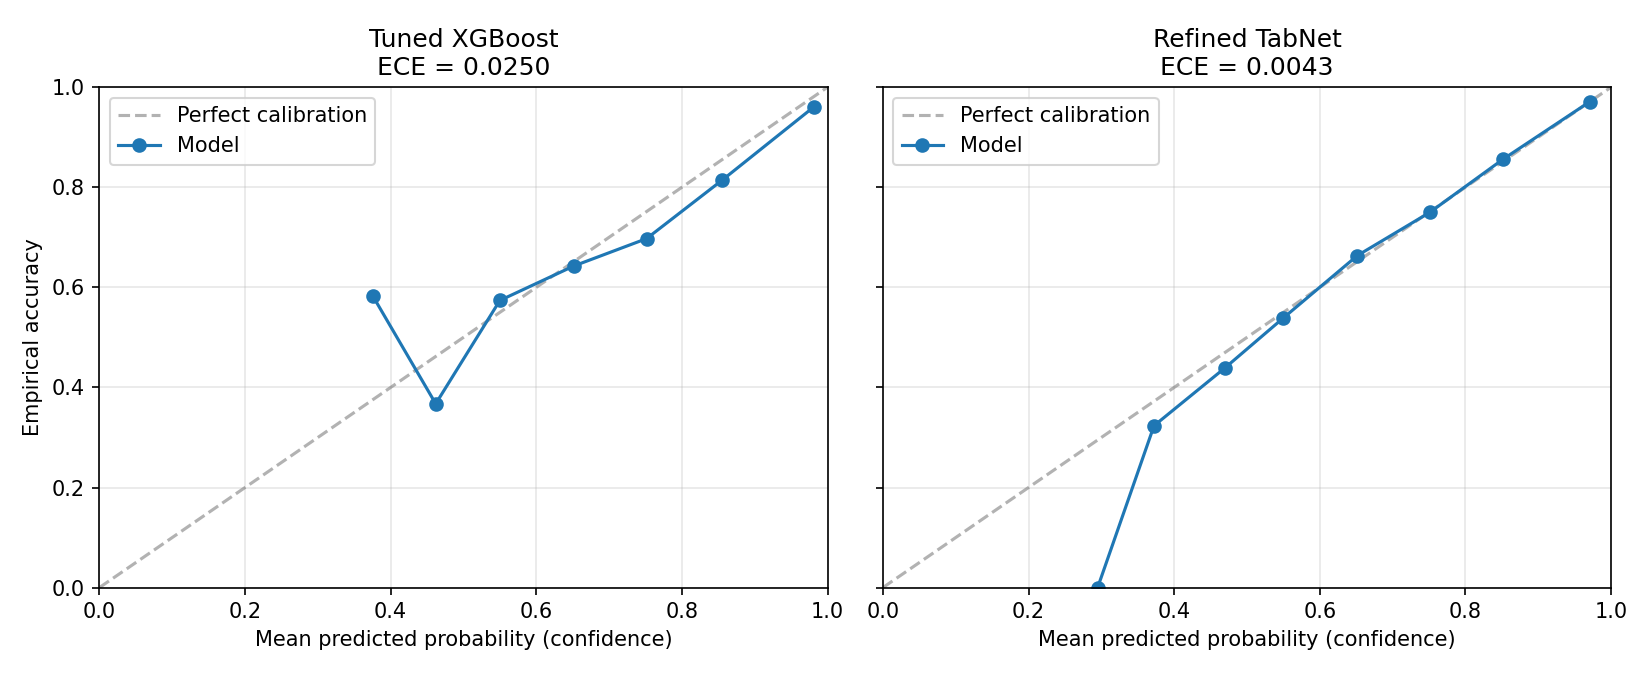
\includegraphics[width=0.6\textwidth]{reliability_diagrams.png}
  \caption{Reliability diagrams on the full random-split test fold,
  before temperature scaling. XGBoost's curve is noisier with a
  downward dip near the 0.45-confidence bin; TabNet's tracks the
  diagonal from its lowest populated bin onward. The diagram does
  not directly visualize the under-confidence story --- that depends
  on \S\ref{sec:audit-proper} and \S\ref{sec:audit-entropy}.}
  \label{fig:reliability}
\end{figure}

\begin{figure}[!htbp]
  \centering
  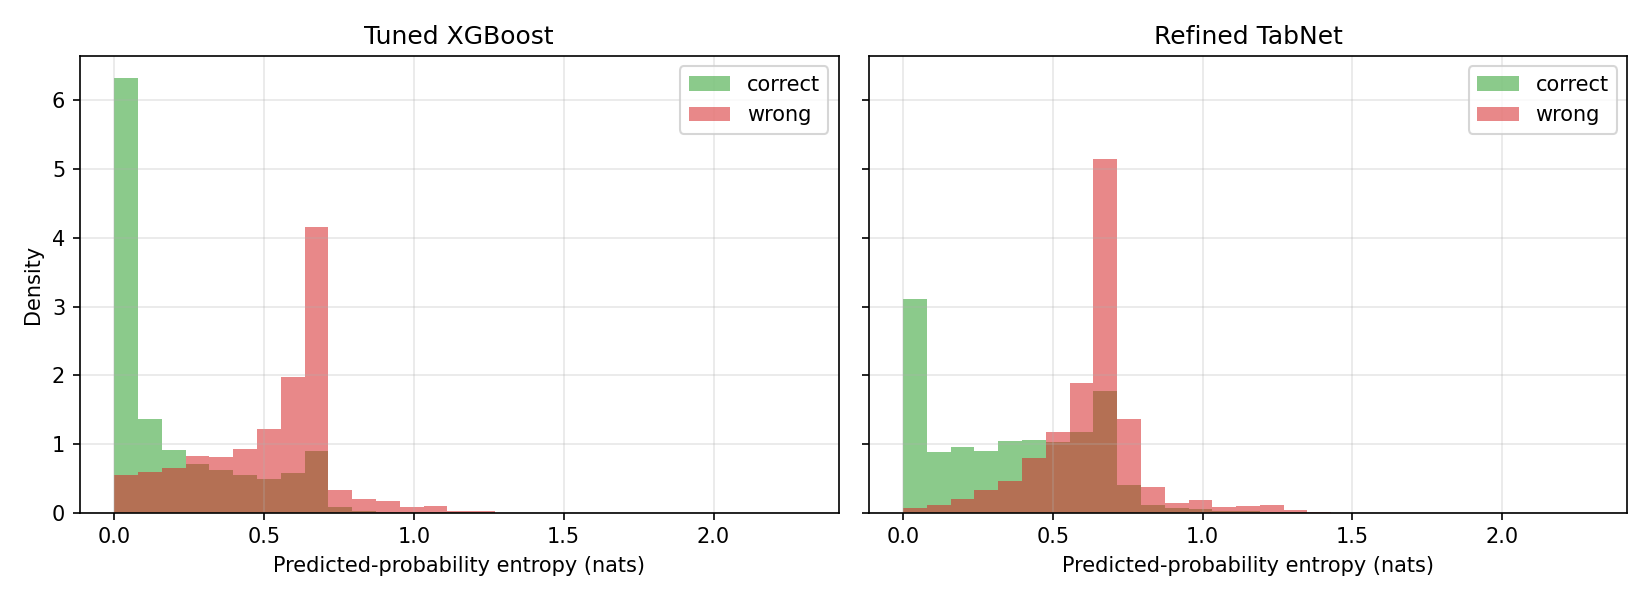
\includegraphics[width=0.5\textwidth]{entropy_correct_vs_incorrect.png}
  \caption{Predicted-distribution entropy histograms, stratified by
  whether the top-1 prediction matched the label. TabNet's
  correct-prediction histogram is shifted right, the graphical
  complement of \S\ref{sec:audit-entropy}.}
  \label{fig:entropy}
\end{figure}

%======================================================================
\section{Error Analysis}\label{sec:errors}

The \S\ref{sec:experiments} numbers and the \S\ref{sec:stats} tests
settle the aggregate question. This section opens up the per-row and
per-class structure. We present the confusion matrices for both
finalized models, examine how their errors overlap row by row, and
read the per-class F1 numbers from the random split alongside the
2023$\rightarrow$2024 temporal split.

\subsection{Confusion matrices}\label{sec:errors-conf}

Figures~\ref{fig:cm-xgb} and~\ref{fig:cm-tabnet} show the
row-normalized confusion matrices for the two finalized models.
Both classify Marine Thunderstorm Wind perfectly (967/967 under
each). The dominant confusion under both is Hail $\leftrightarrow$
Thunderstorm Wind --- Hail recall is 0.737 (XGB) vs 0.630 (TabNet),
with off-diagonal mass concentrated on Thunderstorm Wind. TabNet
also trades Excessive Heat recall (0.675 vs XGB's 0.846) for Heat
recall (0.948 vs 0.862): its softer decision boundary pulls
threshold-adjacent Excessive Heat rows into ordinary Heat.

\subsection{Cross-model error overlap}\label{sec:errors-overlap}

A natural question after \S\ref{sec:stats} is whether the two
models make the \emph{same} errors or \emph{different} ones. The
four-cell agreement table on per-row correctness:

\begin{center}
\small
\begin{tabular}{lrrr}
\toprule
                       & XGBoost correct & XGBoost wrong & row total \\
\midrule
TabNet correct          & 18{,}419 &    908 & 19{,}327 \\
TabNet wrong            &  2{,}283 &  1{,}934 &  4{,}217 \\
column total            & 20{,}702 &  2{,}842 & 23{,}544 \\
\bottomrule
\end{tabular}
\end{center}

The agreement rate is 86.4\%; Cohen's $\kappa = 0.472$. Two
readings. First, the off-diagonal cells are not symmetric. XGBoost
is uniquely correct on 2{,}283 rows where TabNet errs; TabNet is
uniquely correct on only 908 rows where XGBoost errs --- a ratio of
roughly $2.5:1$, consistent with the \S\ref{sec:exp-mf1} \mF{} gap.
Second, $\kappa = 0.47$ sits in the ``moderate'' agreement band of
the Landis-Koch scale. If errors were fully independent at observed
individual accuracy rates, the both-wrong cell would contain
$\sim$509 rows; we observe 1{,}934. Errors are \emph{correlated},
but not redundantly so: $908 + 2{,}283 = 3{,}191$ rows are
correctable by exactly one of the two models. That is the headroom
an ensemble would draw on; \S\ref{sec:discussion} flags this as the
most defensible follow-up.

The per-class breakdown of the overlap
(Figure~\ref{fig:overlap-per-class}) shows the headroom is not
evenly distributed. Hail has 743 XGB-only-correct rows against 299
TabNet-only-correct, and 790 both-wrong rows --- by far the largest
both-wrong cell of any class. Thunderstorm Wind has 795
XGB-only-correct against 327 TabNet-only-correct. The one class
where TabNet is uniquely better than XGBoost on net is Heat: 140
TabNet-only-correct against 29 XGB-only-correct.

\subsection{Per-class F1: random split vs 2023\,$\rightarrow$\,2024}\label{sec:errors-perclass}

Table~\ref{tab:per-class} sets the random-split per-class F1
alongside the temporal-split per-class F1 for both models.

\begin{table}[h]
  \centering
  \scriptsize
  \caption{Per-class F1 under the random split and the
  2023$\rightarrow$2024 temporal split, for both finalized models.
  Bolded rows are the boundary classes the proposal singled out.}
  \label{tab:per-class}
  \begin{tabular}{lrrrrrr}
    \toprule
    class & XGB random & TN random & $\Delta$ random & XGB temporal & TN temporal & $\Delta$ temporal \\
    \midrule
    Drought           & 0.997 & 0.996 & $-0.001$ & 0.979 & 0.969 & $-0.010$ \\
    Excessive Heat    & 0.862 & 0.783 & $-0.079$ & 0.577 & 0.567 & $-0.011$ \\
    Flash Flood       & 0.878 & 0.827 & $-0.052$ & 0.779 & 0.755 & $-0.025$ \\
    Flood             & 0.845 & 0.781 & $-0.065$ & 0.697 & 0.637 & $-0.060$ \\
    \textbf{Hail}     & \textbf{0.761} & \textbf{0.648} & \textbf{$-0.113$} & \textbf{0.554} & \textbf{0.591} & \textbf{$+0.037$} \\
    Heat              & 0.845 & 0.812 & $-0.033$ & 0.587 & 0.651 & $+0.065$ \\
    High Wind         & 0.968 & 0.928 & $-0.041$ & 0.795 & 0.750 & $-0.044$ \\
    Marine TS Wind    & 0.999 & 0.998 & $-0.001$ & 0.995 & 0.993 & $-0.003$ \\
    \textbf{TS Wind}  & \textbf{0.880} & \textbf{0.822} & \textbf{$-0.058$} & \textbf{0.760} & \textbf{0.777} & \textbf{$+0.017$} \\
    Winter Weather    & 0.966 & 0.919 & $-0.046$ & 0.834 & 0.798 & $-0.036$ \\
    \bottomrule
  \end{tabular}
\end{table}

On the random split, TabNet loses on every class. The two losses on
the proposal's named boundary classes --- Hail $-0.113$ and
Thunderstorm Wind $-0.058$ --- are not only in the wrong direction
relative to the proposal's prediction, they are the largest two
losses on the table in absolute terms (after a tie with Excessive
Heat at $-0.079$).

The temporal column tells a different story on exactly the two
boundary classes plus Heat. Hail flips sign: TabNet beats XGBoost by
$+0.037$. Thunderstorm Wind flips sign: TabNet by $+0.017$. Heat
flips by $+0.065$. On every other class XGBoost retains the lead
under shift, which is why the aggregate temporal \mF{} still favors
XGBoost (0.7556 vs 0.7487).

The asymmetry of the random$\rightarrow$temporal drops is the more
diagnostic comparison. On Hail XGBoost loses $-0.207$ F1 against
TabNet's $-0.057$; on Thunderstorm Wind, $-0.120$ vs $-0.045$. On
the two proposal classes, TabNet's degradation under shift is
roughly 3--4$\times$ smaller. The pattern is not universal --- High
Wind and Drought show the opposite ordering --- but the two classes
the proposal \emph{named in advance} are the two where TabNet's
softer representations transfer to the next year visibly better.
This is a substantive qualification worth reporting; it is not a
vindication of the mechanism, and \S\ref{sec:limitations} makes the
single-fold caveat explicit.

\begin{figure}[!htbp]
  \centering
  \begin{minipage}{0.48\textwidth}
    \centering
    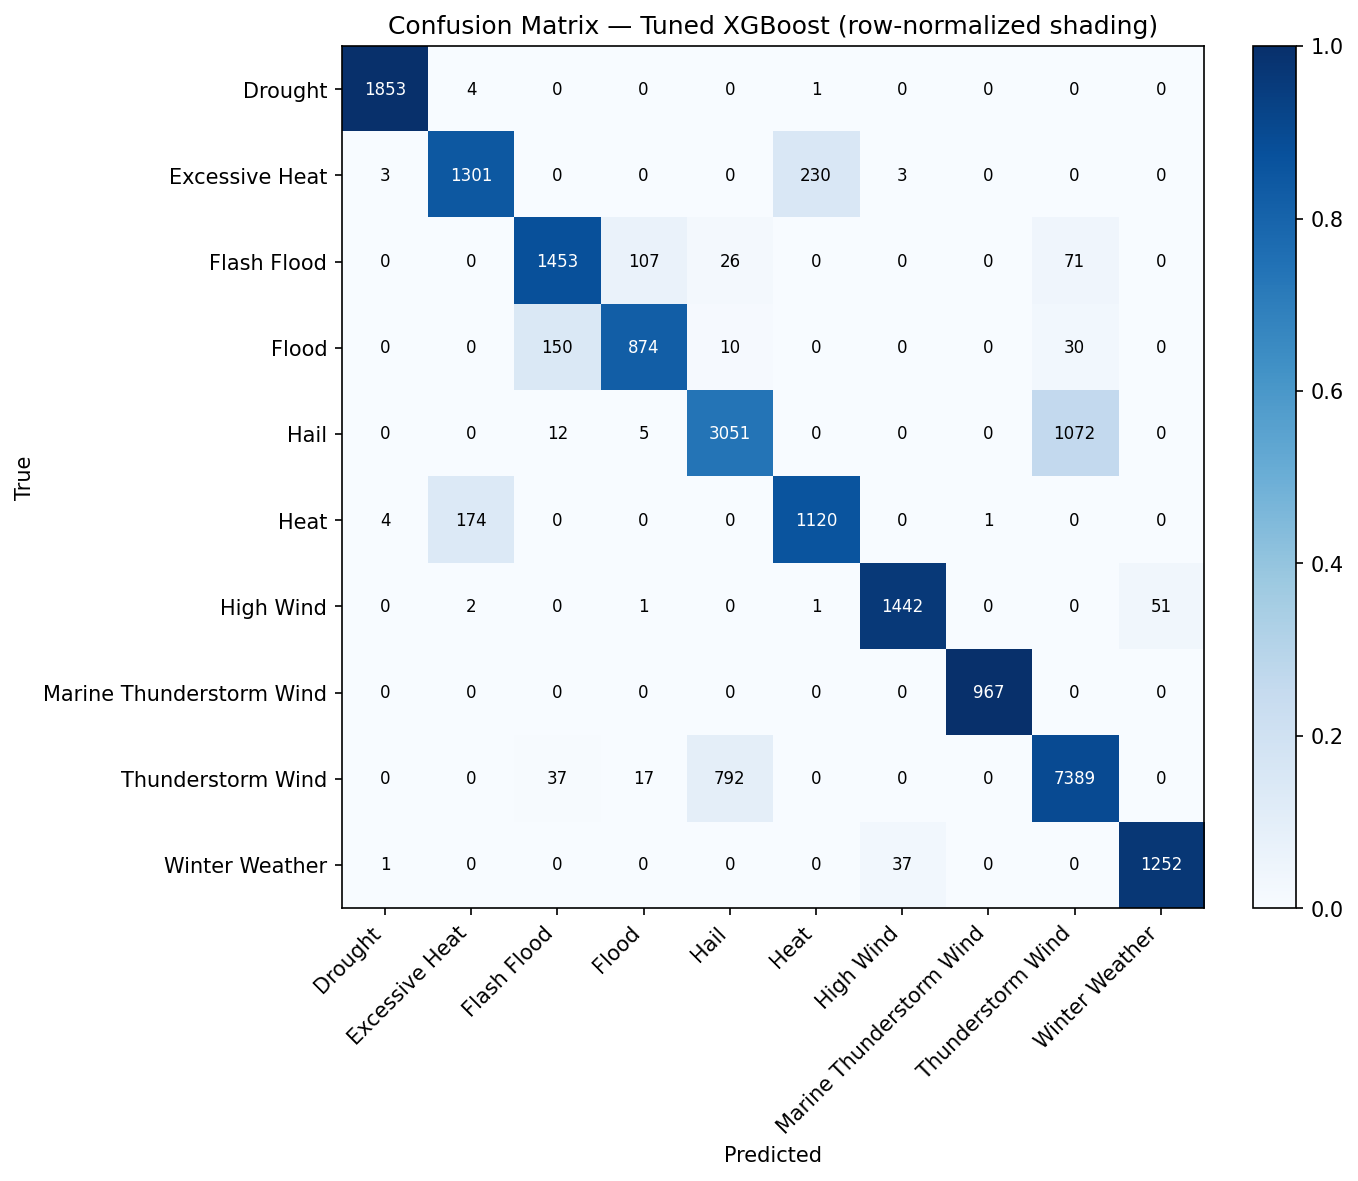
\includegraphics[width=\linewidth]{confusion_matrix_tuned_xgb.png}
    \caption{Confusion matrix, tuned XGBoost.}
    \label{fig:cm-xgb}
  \end{minipage}\hfill
  \begin{minipage}{0.48\textwidth}
    \centering
    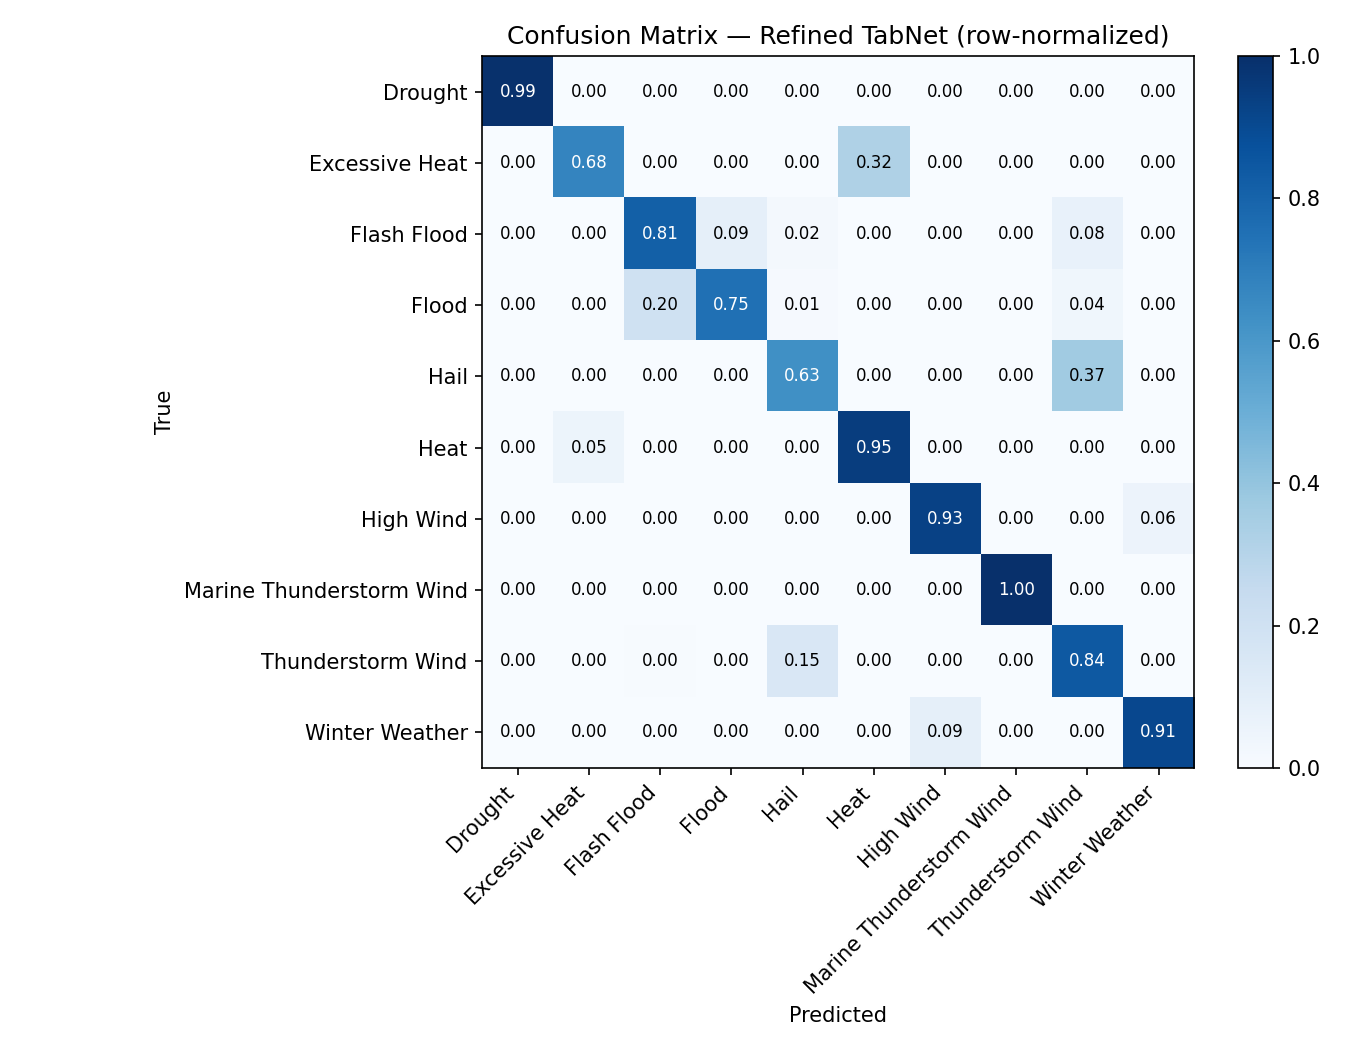
\includegraphics[width=\linewidth]{confusion_matrix_tabnet.png}
    \caption{Confusion matrix, refined TabNet.}
    \label{fig:cm-tabnet}
  \end{minipage}
\end{figure}

\begin{figure}[!htbp]
  \centering
  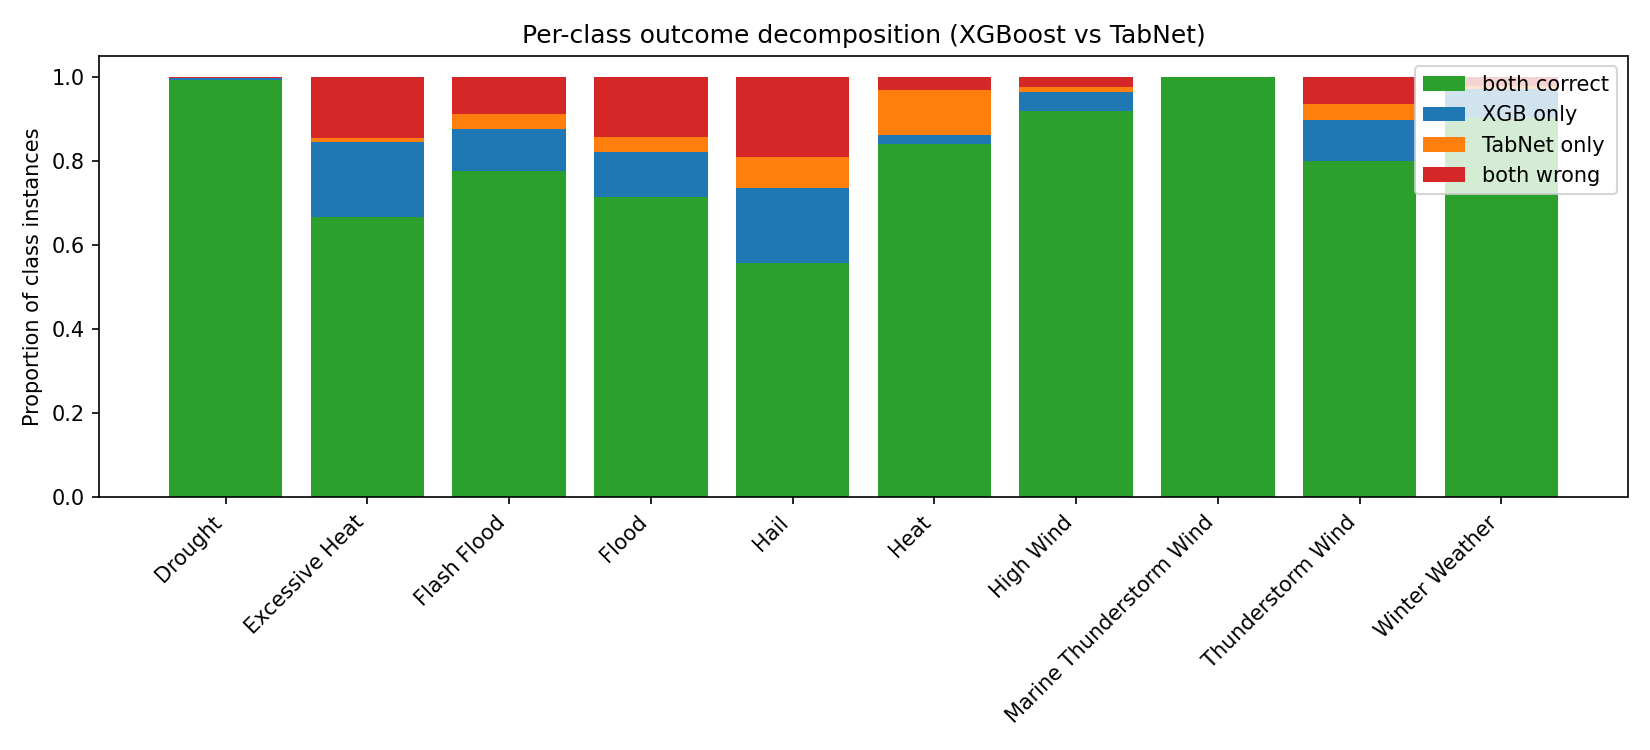
\includegraphics[width=0.7\textwidth]{error_overlap_per_class.png}
  \caption{Per-class breakdown of the four cross-model overlap cells
  (both-correct, XGB-only-correct, TabNet-only-correct, both-wrong).
  Hail dominates the both-wrong cell; Heat is the one class where
  TabNet-only-correct exceeds XGB-only-correct.}
  \label{fig:overlap-per-class}
\end{figure}

\begin{figure}[!htbp]
  \centering
  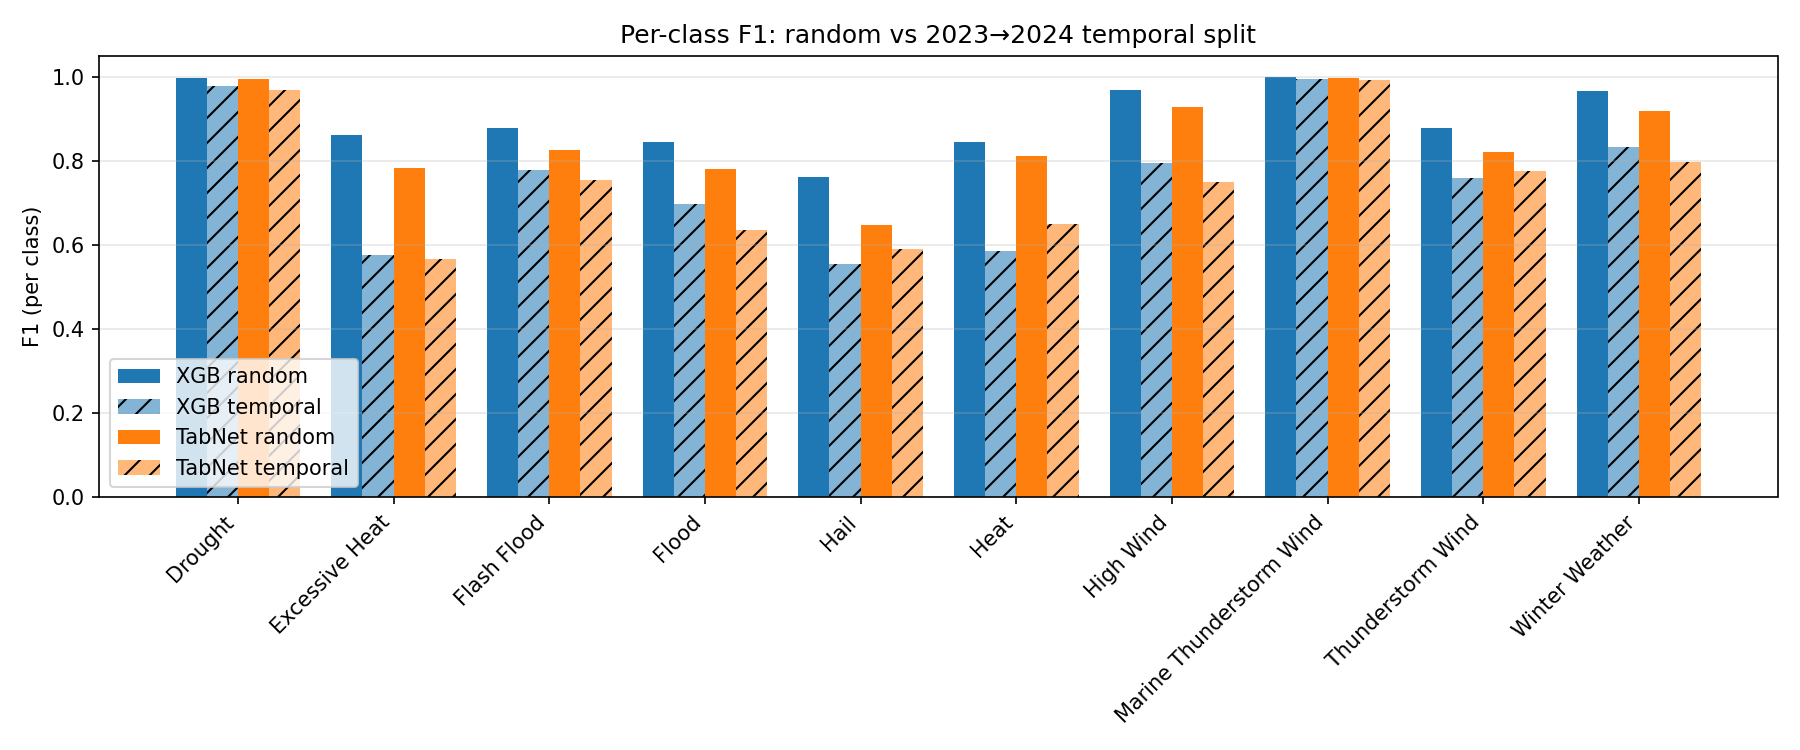
\includegraphics[width=0.65\textwidth]{per_class_f1_random_vs_temporal.png}
  \caption{Per-class F1 under the random split and the
  2023$\rightarrow$2024 temporal hold-out for both finalized models.
  Anchors \S\ref{sec:errors-perclass}.}
  \label{fig:per-class-f1}
\end{figure}

%======================================================================
\section{Interpretability}\label{sec:interp}

When each model makes a prediction, which features is it actually
using? Tabular interpretability has a sharp methodological
asymmetry --- XGBoost exposes a global gain-based importance score
over features, and TabNet exposes per-step attention masks over
features for every input row. The two artifacts are not directly
commensurable, but they can both be reduced to a per-feature score
on the same 8-feature axis.

\paragraph{XGBoost gain-based importance.}

The tuned XGBoost's split-gain importance over the 8 engineered
features:

\begin{center}
\small
\begin{tabular}{lr}
\toprule
feature & gain importance \\
\midrule
\texttt{CZ\_TYPE\_ENC}  & 0.9037 \\
\texttt{DURATION\_MIN}  & 0.0357 \\
\texttt{STATE\_ENC}     & 0.0202 \\
\texttt{MONTH}          & 0.0131 \\
\texttt{WFO\_ENC}       & 0.0080 \\
\texttt{BEGIN\_LON}     & 0.0079 \\
\texttt{HOUR}           & 0.0057 \\
\texttt{BEGIN\_LAT}     & 0.0056 \\
\bottomrule
\end{tabular}
\end{center}

The distribution is extremely concentrated. \texttt{CZ\_TYPE\_ENC}
alone accounts for 90.4\% of total gain; the next feature
(\texttt{DURATION\_MIN}) takes 3.6\%; the remaining six share the
final 6\%. \texttt{CZ\_TYPE\_ENC} is the NOAA county-zone-marine
type code, which lets the model separate Marine Thunderstorm Wind
from its land counterpart at near-perfect accuracy
(\S\ref{sec:errors-conf}). \texttt{DURATION\_MIN} separates
short-duration severe events (Hail, Thunderstorm Wind) from
longer-duration ones (Flood, Winter Weather, Drought).

\paragraph{TabNet attention masks.}\label{sec:interp-tabnet}

TabNet exposes per-step attention masks $M[s, i, f]$ giving the
weight that step $s$ placed on feature $f$ for row $i$ (shape
$7 \times 23{,}544 \times 8$). The row-and-step-averaged importance:

\begin{center}
\small
\begin{tabular}{lr}
\toprule
feature & mean mask weight \\
\midrule
\texttt{CZ\_TYPE\_ENC}  & 0.1912 \\
\texttt{DURATION\_MIN}  & 0.1774 \\
\texttt{HOUR}           & 0.1449 \\
\texttt{BEGIN\_LAT}     & 0.1393 \\
\texttt{BEGIN\_LON}     & 0.1209 \\
\texttt{MONTH}          & 0.0940 \\
\texttt{STATE\_ENC}     & 0.0890 \\
\texttt{WFO\_ENC}       & 0.0433 \\
\bottomrule
\end{tabular}
\end{center}

The shape is qualitatively different from XGBoost's.
\texttt{CZ\_TYPE\_ENC} is still in first place, but with only 19\%
of total mask mass instead of XGBoost's 90\% --- and the tail does
not collapse. The least-used feature (\texttt{WFO\_ENC}) still
receives 4.3\% of total mask weight. A per-row TabNet prediction is
built from contributions of all eight features at non-trivial
weight.

The step-wise decomposition shows that each of TabNet's seven steps
specializes on a different feature subset: step 5 allocates 62\% of its mask weight to
\texttt{DURATION\_MIN} alone; step 2 is a latitude/longitude step;
step 4 is an hour-of-day step; \texttt{CZ\_TYPE\_ENC} is in the
top-4 of every step. The architecture is recognizable as
feature-selecting in the way \citet{arik2021tabnet} describe --- but
on this 8-feature task it never has enough irrelevant features to
filter away. The local-attribution explain matrix, which weights
per-step masks by each step's contribution to the prediction,
re-ranks the top two: mean $|\mathrm{explain}|$ puts
\texttt{DURATION\_MIN} (4.24) ahead of \texttt{CZ\_TYPE\_ENC} (2.88),
because step~5's heavy \texttt{DURATION\_MIN} allocation carries
large prediction weight despite a marginal mask share of only
17.7\%. \texttt{WFO\_ENC} is last under either ranking (0.94).

\paragraph{Cross-model comparison.}\label{sec:interp-compare}

Reduced to ranks on the common 8-feature axis, the two models agree
much more than the distribution shapes suggest.

\begin{center}
\small
\begin{tabular}{lrrr}
\toprule
feature & XGB rank (gain) & TN rank (mask) & TN rank ($|\mathrm{explain}|$) \\
\midrule
\texttt{CZ\_TYPE\_ENC}  & 1 & 1 & 2 \\
\texttt{DURATION\_MIN}  & 2 & 2 & 1 \\
\texttt{STATE\_ENC}     & 3 & 7 & 7 \\
\texttt{MONTH}          & 4 & 6 & 3 \\
\texttt{WFO\_ENC}       & 5 & 8 & 8 \\
\texttt{BEGIN\_LON}     & 6 & 5 & 5 \\
\texttt{HOUR}           & 7 & 3 & 4 \\
\texttt{BEGIN\_LAT}     & 8 & 4 & 6 \\
\bottomrule
\end{tabular}
\end{center}

The two top features (\texttt{CZ\_TYPE\_ENC},
\texttt{DURATION\_MIN}) are the top-two under all three rankings;
the bottom feature (\texttt{WFO\_ENC}) is in the bottom-two under
all three. The middle ordering disagrees --- XGBoost places
\texttt{STATE\_ENC} third but TabNet places it seventh; TabNet
places \texttt{HOUR} and \texttt{BEGIN\_LAT} in its top half but
XGBoost places them seventh and eighth. The discrepancy reflects an
architectural difference: XGBoost encodes location through
\texttt{STATE\_ENC} because boosted trees split repeatedly on that
integer-coded category, while TabNet's masks distribute location
information across the raw lat/lon features instead. Both models
are solving the same problem with the same information; they
package the location signal differently.

The agreement at the top and bottom of the ranking is the
load-bearing observation for \S\ref{sec:discussion}. Both models
converge on a feature subset of roughly two strong features and six
weaker but non-negligible features. There is no ``irrelevant''
feature for TabNet's attention to filter out --- the worst feature
on this task (\texttt{WFO\_ENC}) still earns 4.3\% of TabNet's mask
weight and 0.8\% of XGBoost's gain.

\begin{figure}[!htbp]
  \centering
  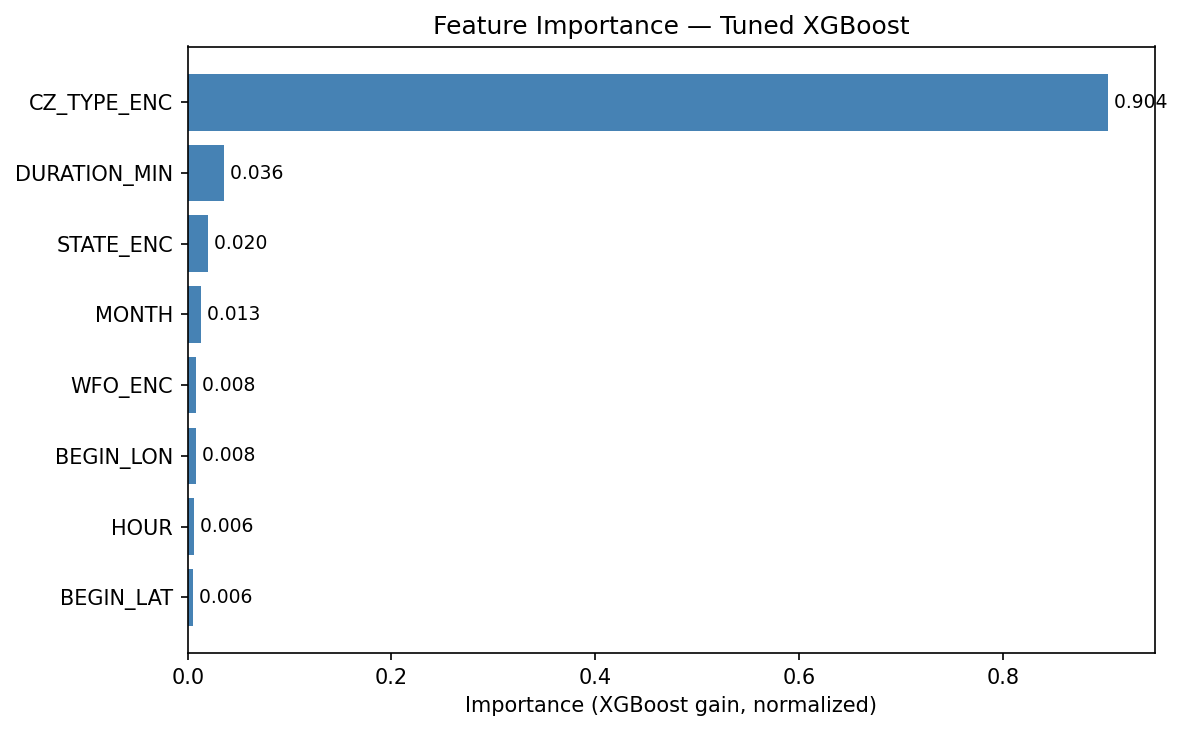
\includegraphics[width=0.5\textwidth]{feature_importance_tuned_xgb.png}
  \caption{Tuned-XGBoost split-gain importance over the 8 engineered
  features. The visual emphasizes the 90\%-on-\texttt{CZ\_TYPE\_ENC}
  concentration.}
  \label{fig:fi-xgb}
\end{figure}


%======================================================================
\section{Discussion}\label{sec:discussion}

The empirical sections leave three things to explain: why the
random-split \mF{} result came out against the pre-registered
hypothesis, why the 2023$\rightarrow$2024 temporal split partially
recovers it on exactly the two named boundary classes, and what to
do with the moderate cross-model error independence we measured in
\S\ref{sec:errors-overlap}.

\paragraph{Why XGBoost wins the random split.}\label{sec:disc-why}
TabNet's architectural promise is sparse, instance-adaptive feature
selection regularized by a sparsity prior $\gamma$
\citep{arik2021tabnet}. The mechanism is most valuable when
\emph{selection itself} is the hard part of the problem --- when the
input has many redundant or irrelevant features. On our 8-feature
working set, selection is not the hard part: even the worst feature
(\texttt{WFO\_ENC}) receives 4.3\% of TabNet's mask weight and 0.8\%
of XGBoost's gain, so there is no idle feature for attention to
filter away. This is exactly the regime \citet{shwartz2022tabular}
flag as least favorable for attention-based methods. In that regime
the gradient-boosted baseline is at its strongest: with only 8
features XGBoost's greedy gain-maximization is close to exhaustive.
The negative result is not that TabNet's attention failed
(\S\ref{sec:interp-tabnet} shows it learned coherent
step-specialized masks) but that its comparative advantage requires
a feature regime this dataset does not provide.

\paragraph{Why the temporal qualification is consistent with the mechanism.}
TabNet beats XGBoost on Hail ($+0.037$) and Thunderstorm Wind
($+0.017$) under 2023$\rightarrow$2024 shift, degrading 3--4$\times$
less than XGBoost on those classes. The \S\ref{sec:audit} audit
makes a mechanistic reading available: TabNet produces softer,
less-confident decision boundaries
(\S\ref{sec:audit-proper}, \S\ref{sec:audit-entropy}). A tight,
sharply-confident fit to 2023 pays the largest penalty under
distribution shift in boundary regions, which is where the two
proposal-named classes live; XGBoost's random-to-temporal drops
($-0.207$ Hail, $-0.120$ TS Wind) dwarf TabNet's ($-0.057$,
$-0.045$). We offer this as a hypothesis of mechanism, not a proven
claim --- one annual fold is too thin
(\S\ref{sec:limitations}).

\paragraph{Cross-model error independence and the ensemble follow-up.}
\S\ref{sec:errors-overlap} measured Cohen's $\kappa = 0.47$:
3{,}191 of 23{,}544 test rows are correctable by exactly one of the
two models. A confidence-weighted ensemble would in principle close
some of that gap, with Hail (790 both-wrong) the smallest-headroom
class. We do not run that experiment here; it is the most
defensible follow-up.

%======================================================================
\section{Limitations}\label{sec:limitations}

Four limitations bound the scope of the claim.
\textbf{(i)~Feature count:} our 8-feature engineered working set is
the very regime in which TabNet's selection mechanism has nothing
to filter; the negative result does not transfer mechanically to
wider tabular tasks where only a handful of many features carry
signal. \textbf{(ii)~Single-year temporal fold:} the
2023$\rightarrow$2024 per-class flip on Hail and Thunderstorm Wind
is suggestive but one annual fold cannot support a domain-adaptation
claim; a leave-one-year-out design across multiple NOAA archives
would be the right next step. \textbf{(iii)~No ensemble baseline:}
$\kappa = 0.47$ leaves room for a confidence-weighted ensemble, but
we did not evaluate one. \textbf{(iv)~ECE binning sensitivity:} we
used 10 equal-width bins per \citet{guo2017calibration}, fixed
before the audit; the audit's load-bearing numbers (Brier, NLL,
post-temperature-scaling ECE) are not materially bin-dependent,
which is part of why the audit is robust where ECE alone is not.

%======================================================================
\section{Conclusion}\label{sec:conclusion}

We pre-registered the hypothesis that TabNet's sequential attention
would outperform a tuned gradient-boosted baseline on NOAA Storm
Events 2023 --- and on the principal random-split, iid evaluation,
the hypothesis is falsified along every axis we tested. Tuned
XGBoost beats refined TabNet by $+0.049$ \mF{} (95\% bootstrap CI
$[+0.044, +0.054]$; McNemar $\chi^2 = 591.6$, $p < 10^{-130}$), and
the direction is reversed on exactly the two boundary classes the
proposal singled out. A surface reading of Expected Calibration
Error initially favored TabNet, but a three-control audit --- proper
scoring rules, temperature scaling, and argmax invariance ---
overturned that reading: XGBoost is strictly better under Brier and
NLL, and a single learned scalar $T = 1.26$ makes XGBoost the
better-calibrated model on ECE as well. The one nuance we report
honestly is the 2023$\rightarrow$2024 temporal fold, where TabNet's
softer fit degrades 3--4$\times$ less than XGBoost's on Hail and
Thunderstorm Wind, partially recovering the proposal's per-class
prediction. The broader methodological takeaway is the audit
itself: ECE-only calibration claims in the tabular-DL literature
should be paired with at least one proper scoring rule and a
temperature-scaling baseline before they are believed.

%======================================================================
\bibliography{references}

\end{document}
